\section{推力性质}

\subsection{需用推力$T_R$}

在计算需用推力的$T_R$时,
可以采用如下步骤.
首先给定巡航高度$h$的时候,
可以通过前述的大气模型计算当地大气密度$\rho$和声速$c$。

在巡航时假设飞行器质量为$m$不变,不考虑巡航高度对重力加速度$g$的影响,
可以认为正常巡航时升力等于重力$L = W = mg$。

在飞行马赫数$Ma$给定时,
可以通过升力计算公式计算得到升力系数$C_L$:
\begin{equation}
    C_L = \frac{2W}{ \rho Ma^2 c^2 S }
\end{equation}

通过前节中图\ref{不同马赫数下的零升阻力因子关系}
和图\ref{不同马赫数下的升至阻力因子系数关系}中,
通过样条插值的方式,
可以计算得到在该马赫数$Ma$下的$C_{D0}$和$A$,
进而得到阻力系数:
\begin{equation}
    C_D = C_{D0}(Ma) + A(Ma) C_L^2
\end{equation}

则在此高度$h$下以马赫数$Ma$飞行状况下的需用推力可以计算得到需用推力$T_R$:
\begin{equation}
    T_R = D = \frac{W\cdot C_D}{C_L}
\end{equation}

按上述方法可以绘制不同高度以及飞行马赫数下的需用推力$T_R$如图\ref{不同高度及飞行马赫数下的需用推力}所示。
随高度增加,整个曲线向右下侧“弯腰”。

\begin{figure}[H]
    \centering
    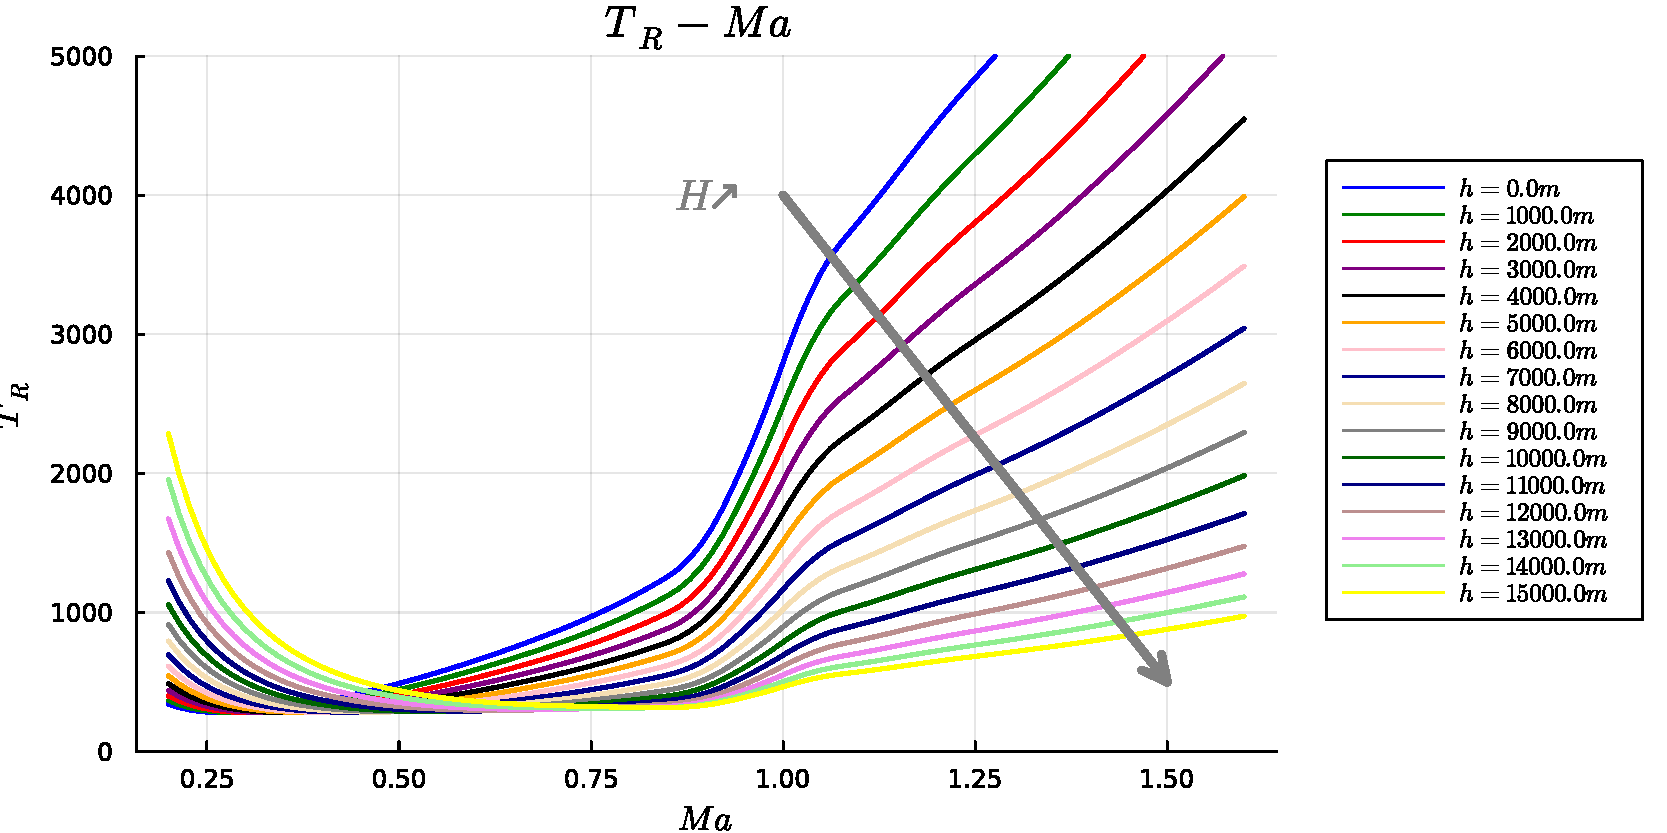
\includegraphics[width=0.8\textwidth]{image/ch4/H_TR_Ma.pdf}
    \caption{不同高度及飞行马赫数下的需用推力$T_R$}
    \label{不同高度及飞行马赫数下的需用推力}
\end{figure}


\subsection{可用推力$T_a$}

可用推力$T_a$总体上取决于发动机本身的性质,
但随着海拔升高,
空气密度降低,
可用推力整体呈下降趋势。
另外,随着飞行马赫数变化,
可用推力曲线也会发生变化。

在给定的数据点中,仅有部分马赫数下的可用推力值,
且有加力(AB)与不加力两个状态,
因此运用样条插值进行外插操作,
在不同巡航高度上,
绘制不同马赫数下的可用推力曲线。

\begin{figure}[H]
    \centering
    \subfloat[$h=0km$]{
        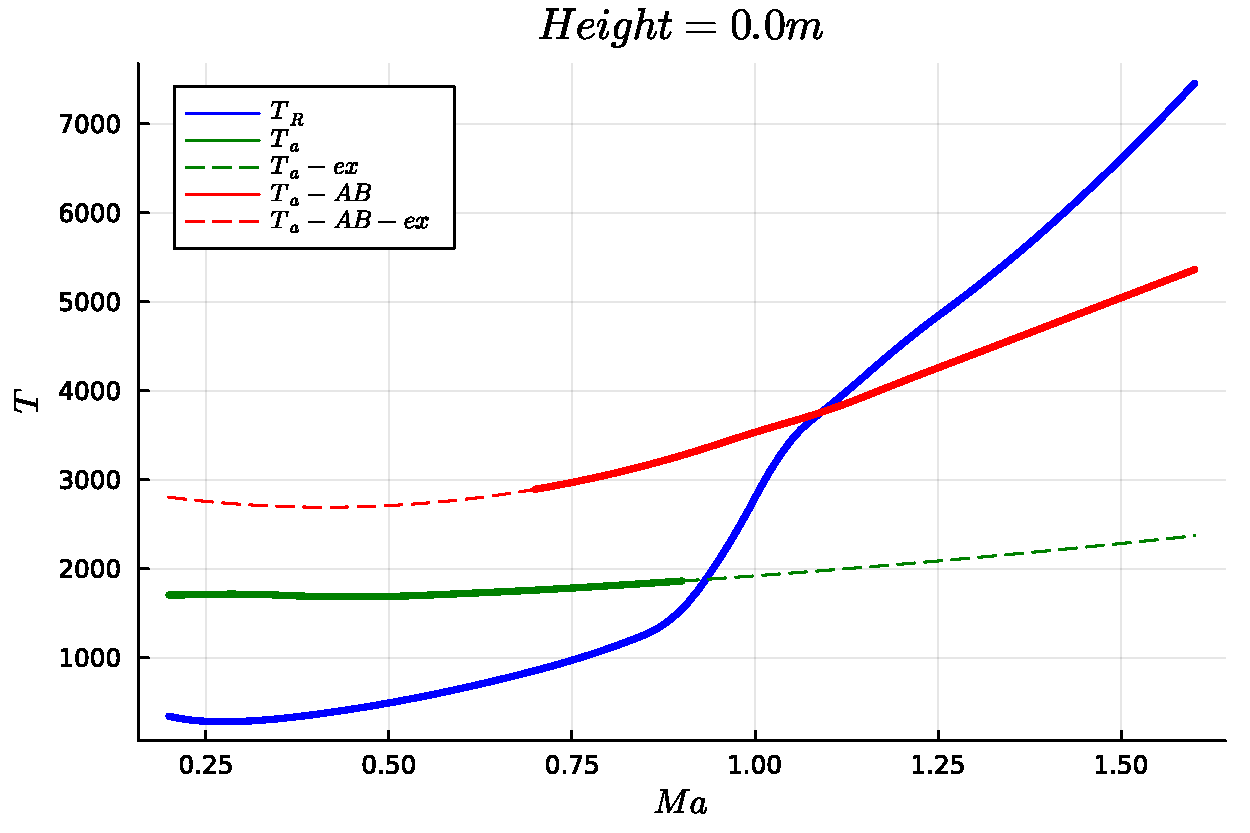
\includegraphics[width=0.25\textwidth]{image/ch4/h_TaTR_Ma1.pdf}
    }
    \subfloat[$h=1km$]{
        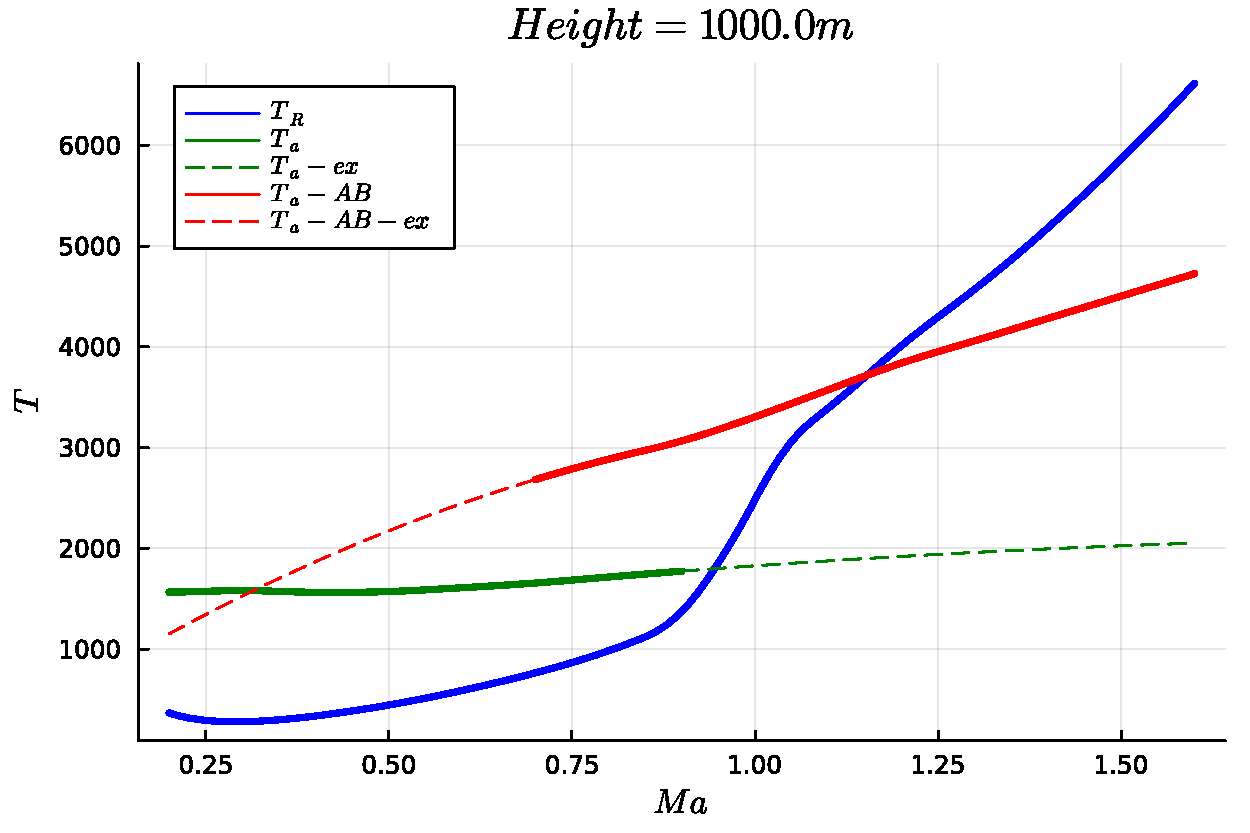
\includegraphics[width=0.25\textwidth]{image/ch4/h_TaTR_Ma2.pdf}
    }
    \subfloat[$h=2km$]{
        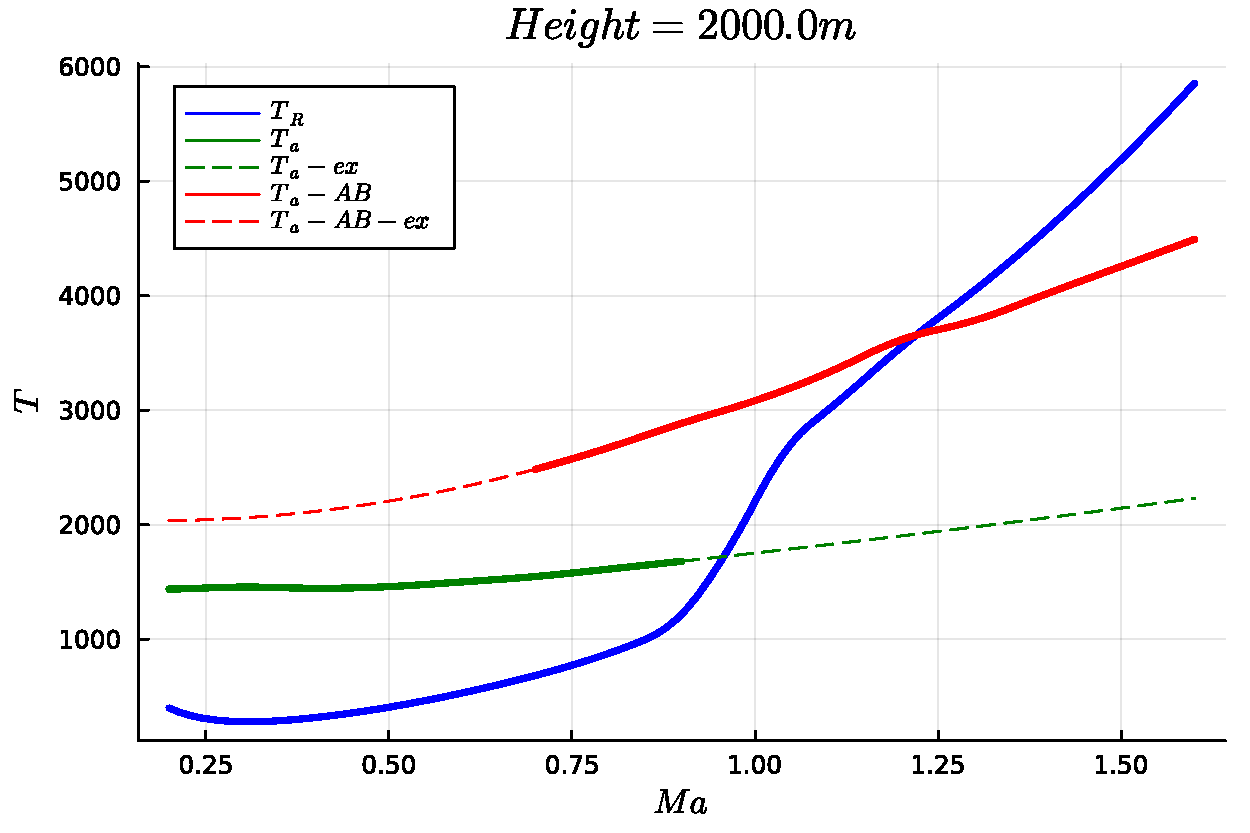
\includegraphics[width=0.25\textwidth]{image/ch4/h_TaTR_Ma3.pdf}
    }
    \subfloat[$h=3km$]{
        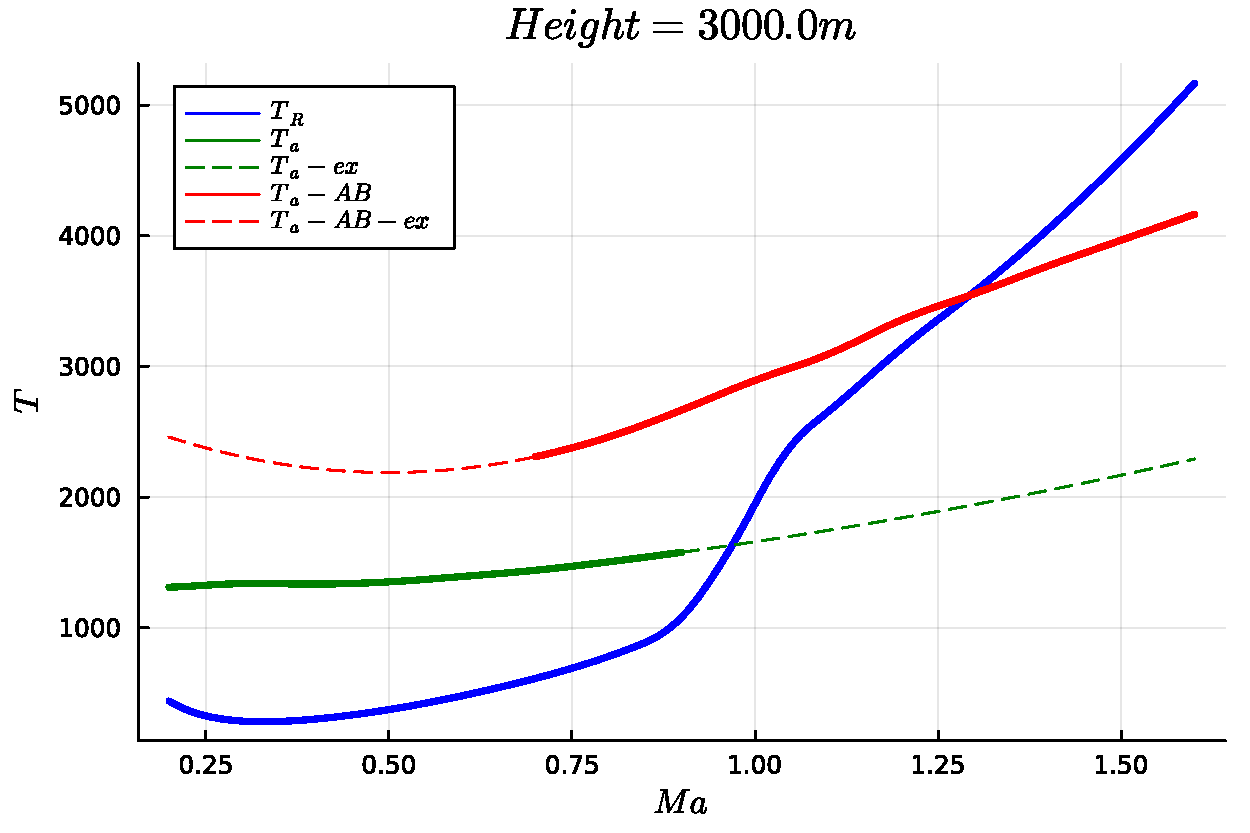
\includegraphics[width=0.25\textwidth]{image/ch4/h_TaTR_Ma4.pdf}
    }
    \quad
    \subfloat[$h=4km$]{
        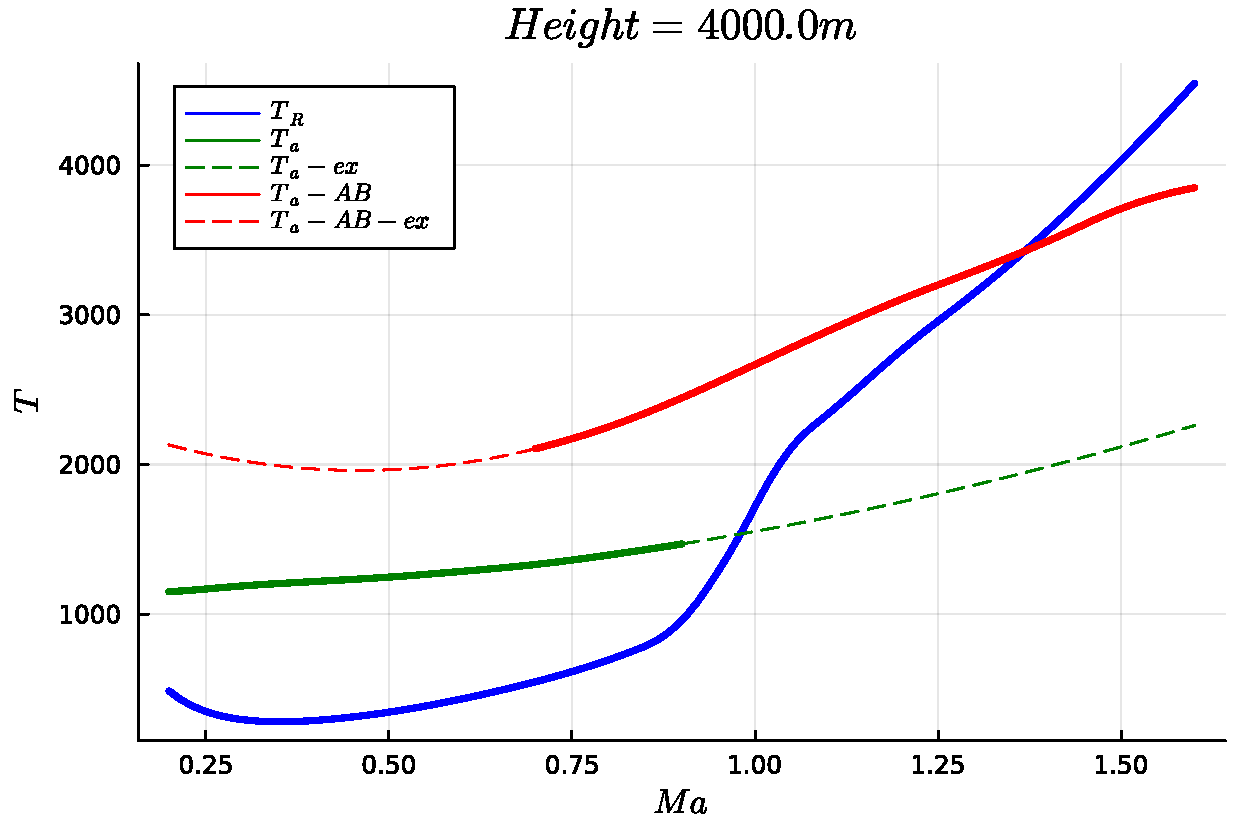
\includegraphics[width=0.25\textwidth]{image/ch4/h_TaTR_Ma5.pdf}
    }
    \subfloat[$h=5km$]{
        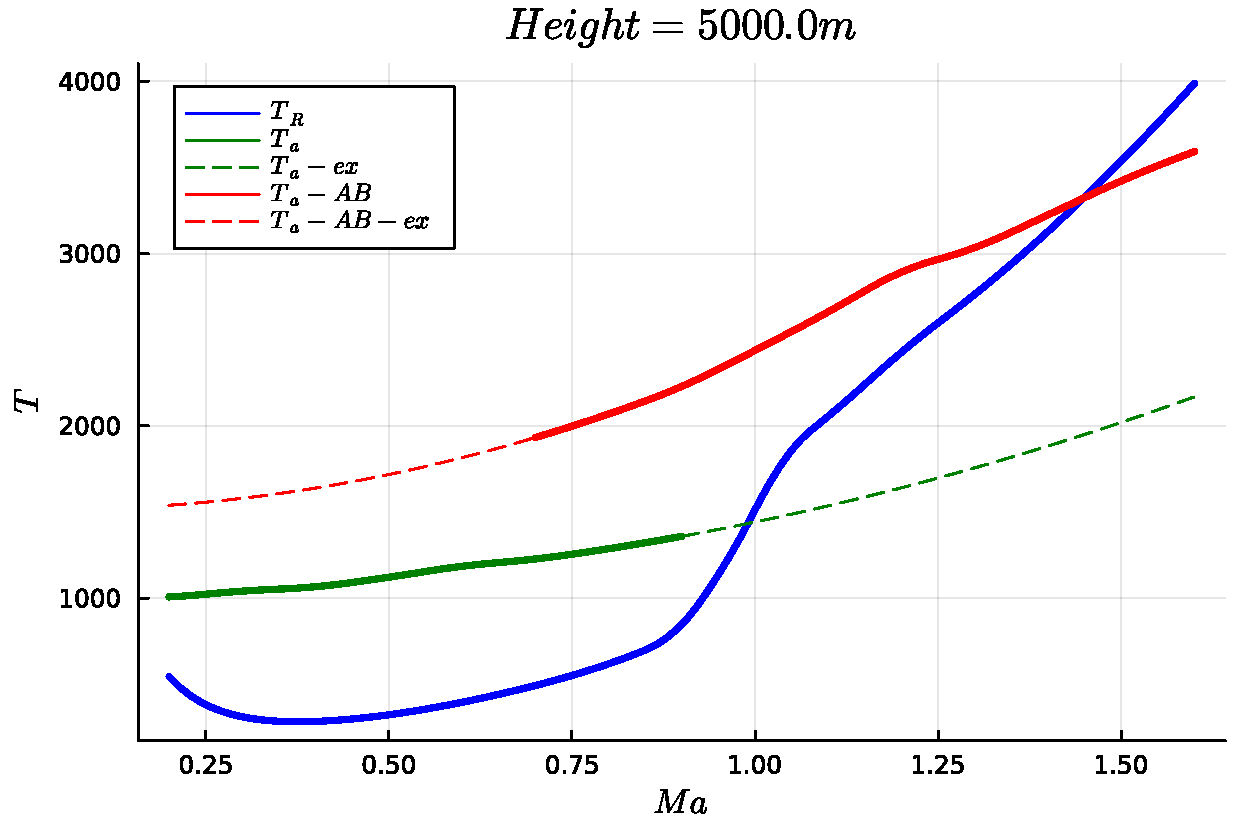
\includegraphics[width=0.25\textwidth]{image/ch4/h_TaTR_Ma6.pdf}
    }
    \subfloat[$h=6km$]{
        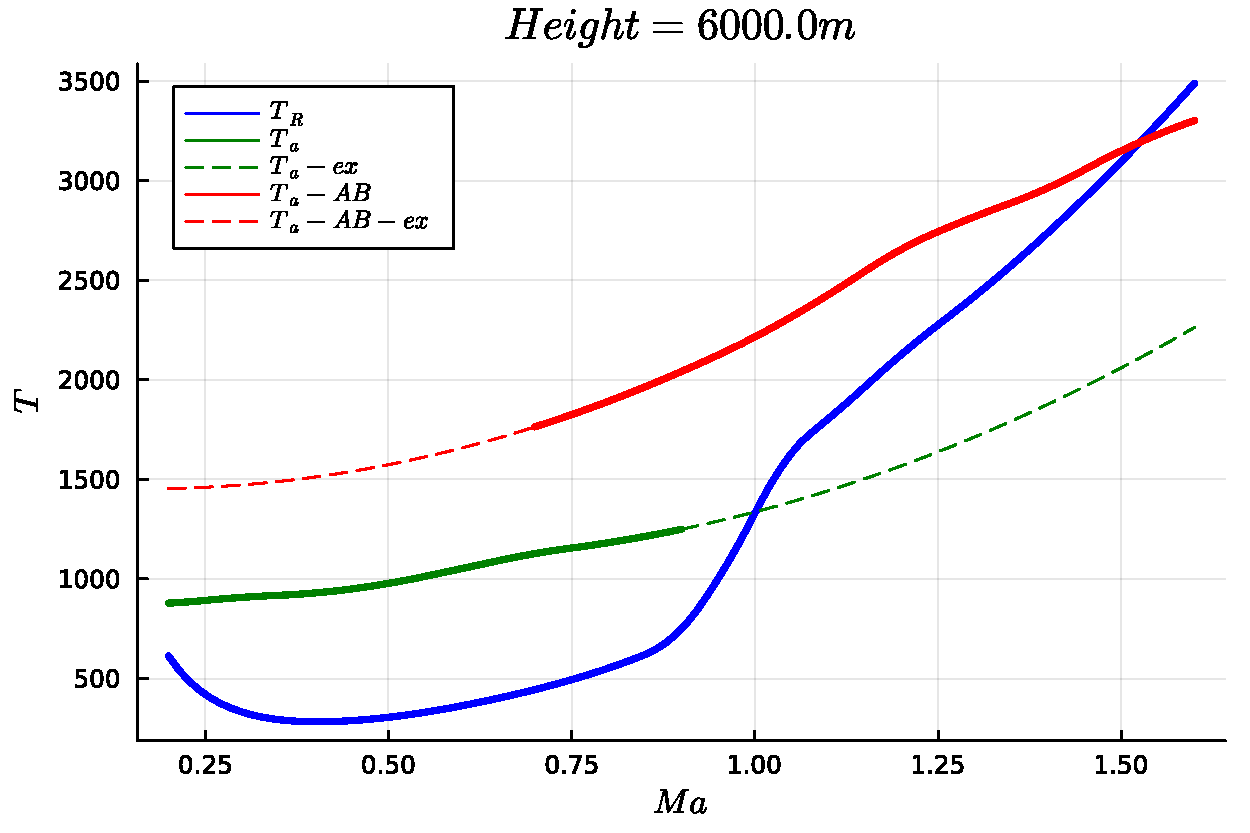
\includegraphics[width=0.25\textwidth]{image/ch4/h_TaTR_Ma7.pdf}
    }
    \subfloat[$h=7km$]{
        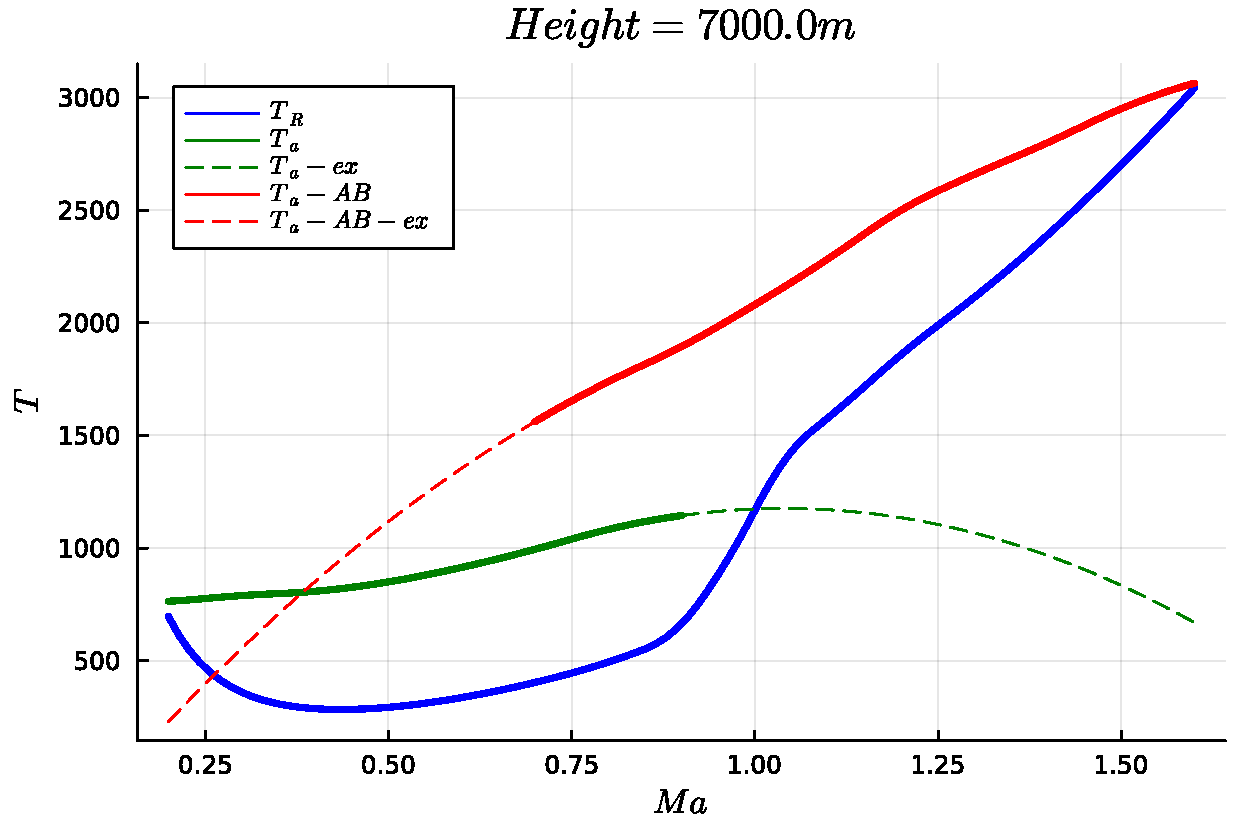
\includegraphics[width=0.25\textwidth]{image/ch4/h_TaTR_Ma8.pdf}
    }
    \quad
    \subfloat[$h=8km$]{
        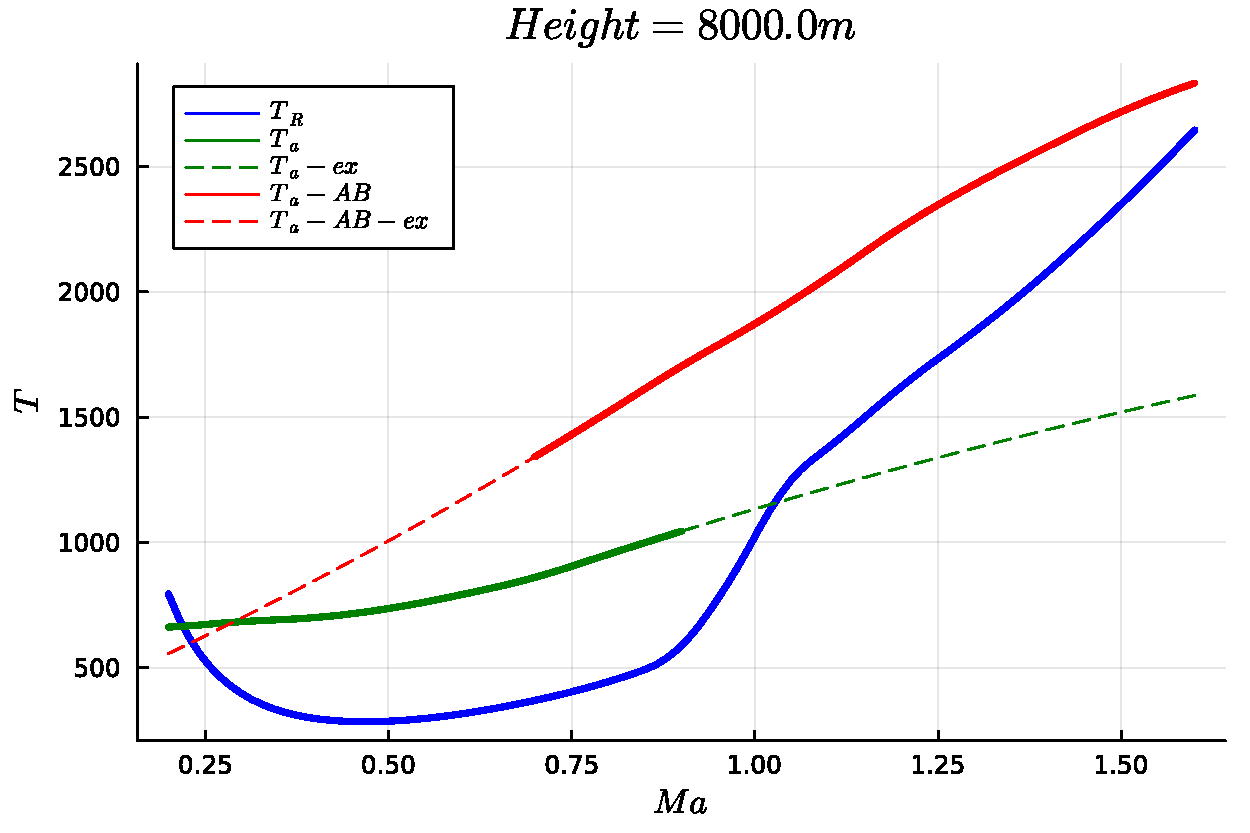
\includegraphics[width=0.25\textwidth]{image/ch4/h_TaTR_Ma9.pdf}
    }
    \subfloat[$h=9km$]{
        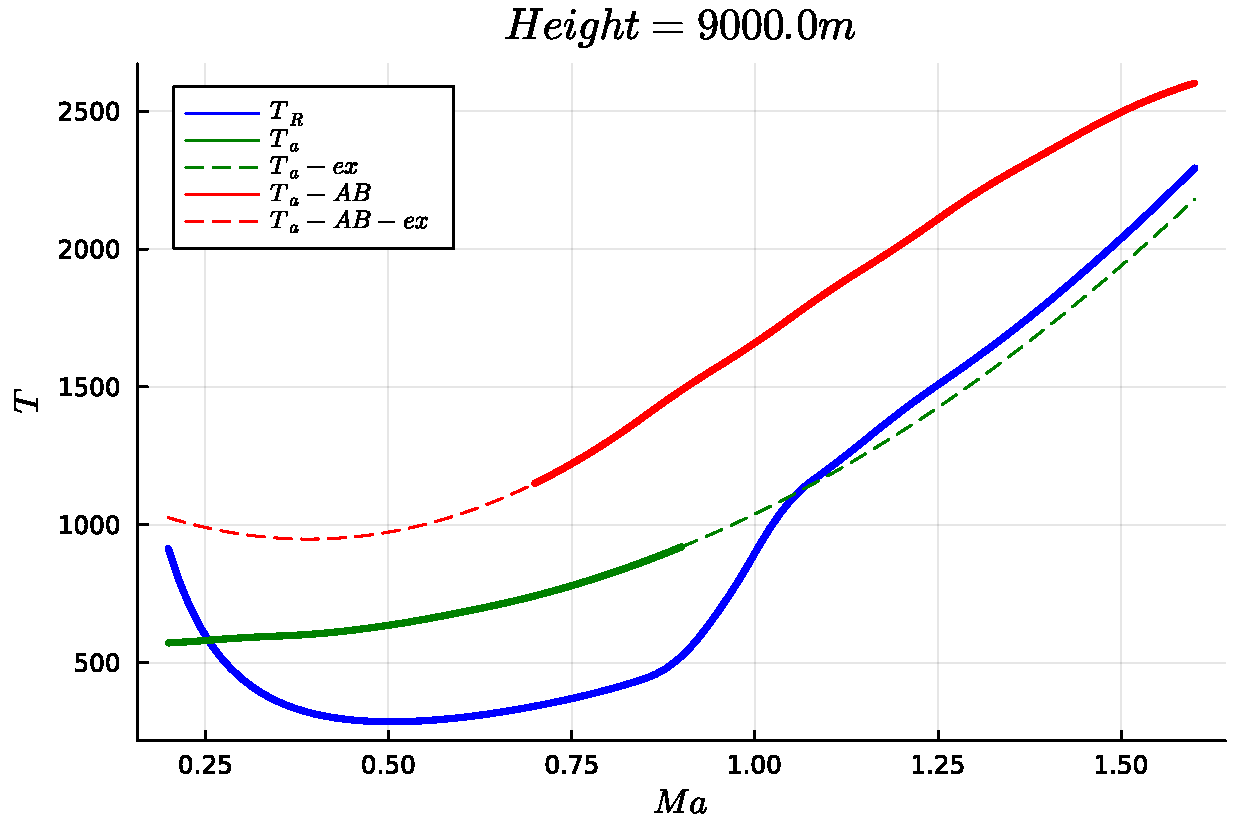
\includegraphics[width=0.25\textwidth]{image/ch4/h_TaTR_Ma10.pdf}
    }
    \subfloat[$h=10km$]{
        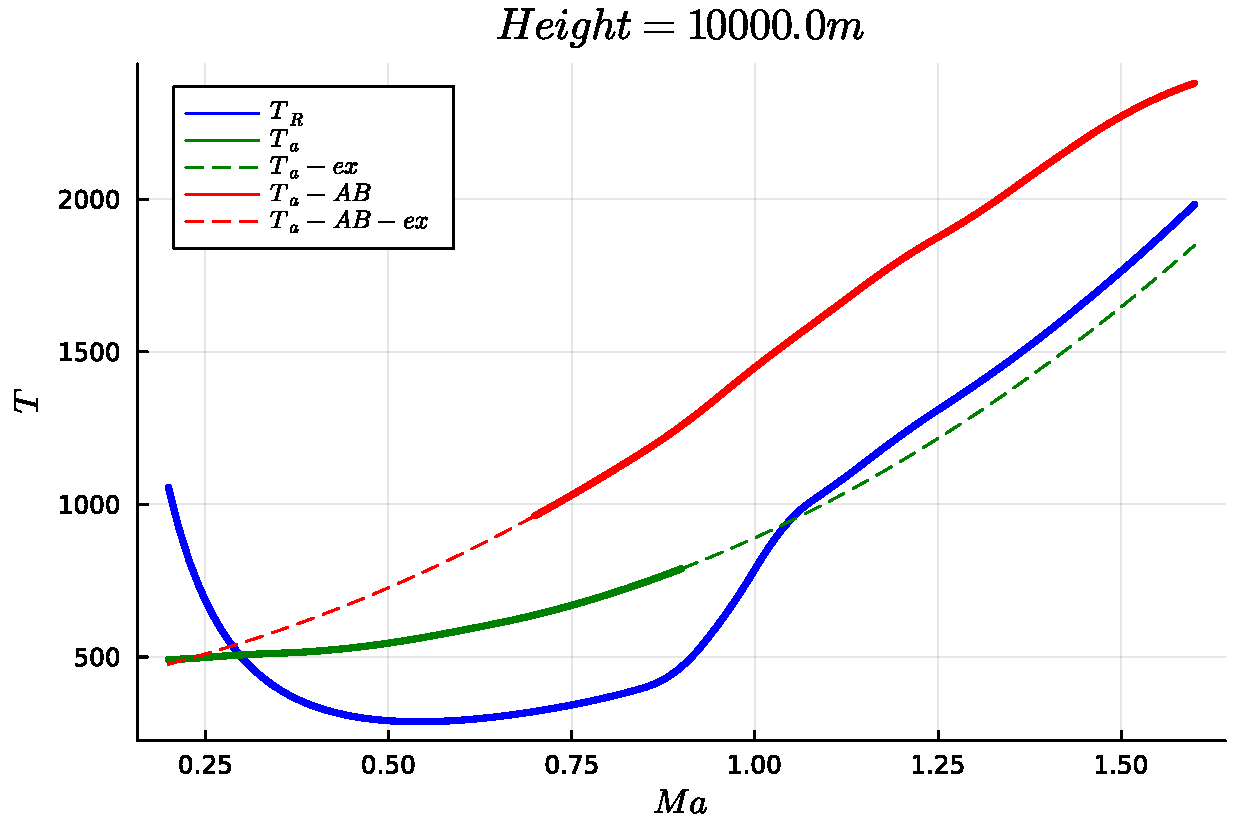
\includegraphics[width=0.25\textwidth]{image/ch4/h_TaTR_Ma11.pdf}
    }
    \subfloat[$h=11km$]{
        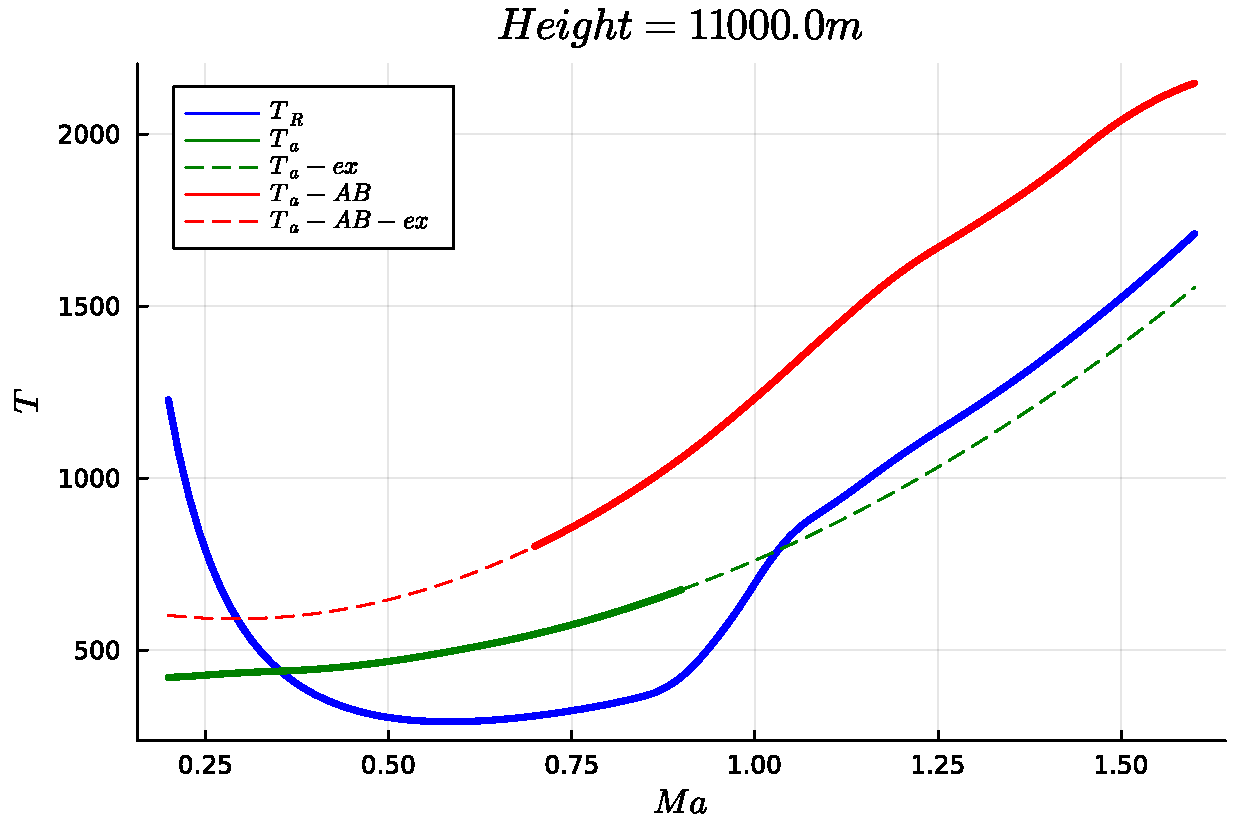
\includegraphics[width=0.25\textwidth]{image/ch4/h_TaTR_Ma12.pdf}
    }
    \quad
    \subfloat[$h=12km$]{
        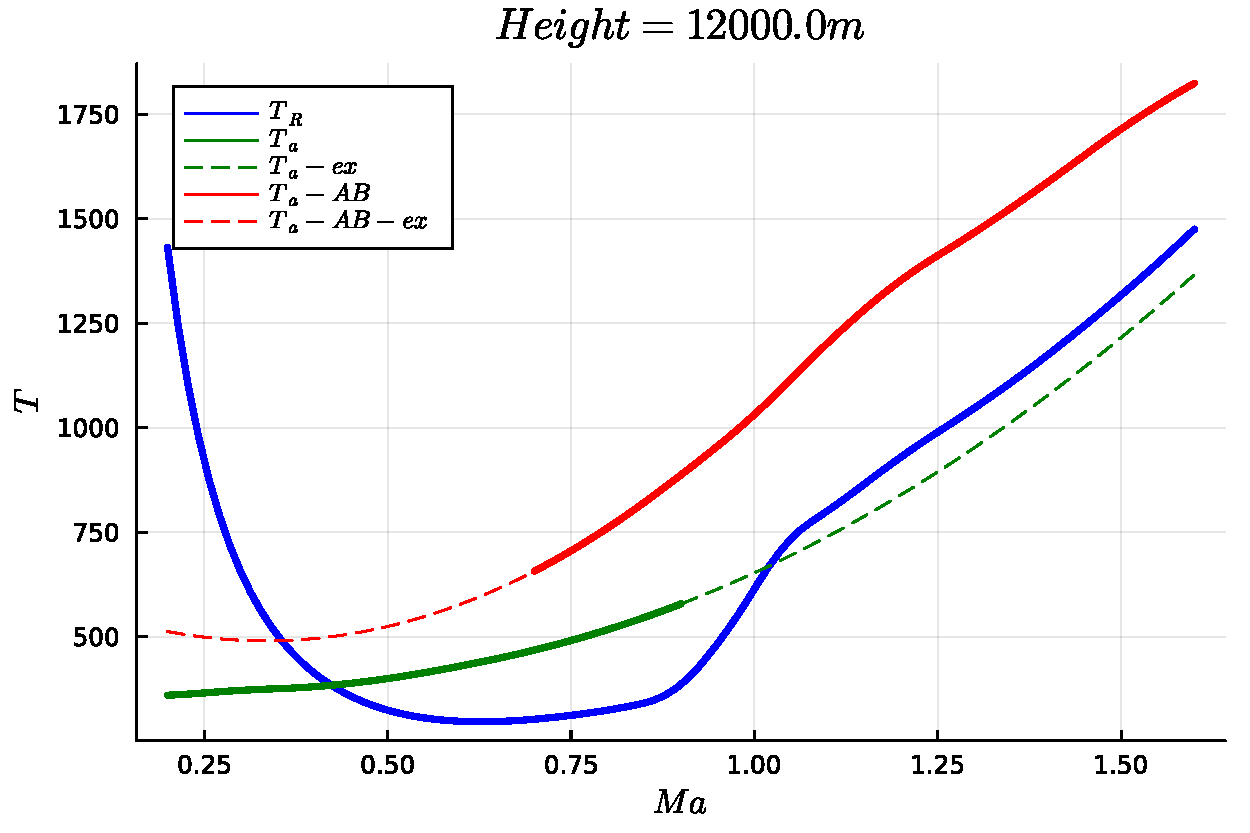
\includegraphics[width=0.25\textwidth]{image/ch4/h_TaTR_Ma13.pdf}
    }
    \subfloat[$h=3km$]{
        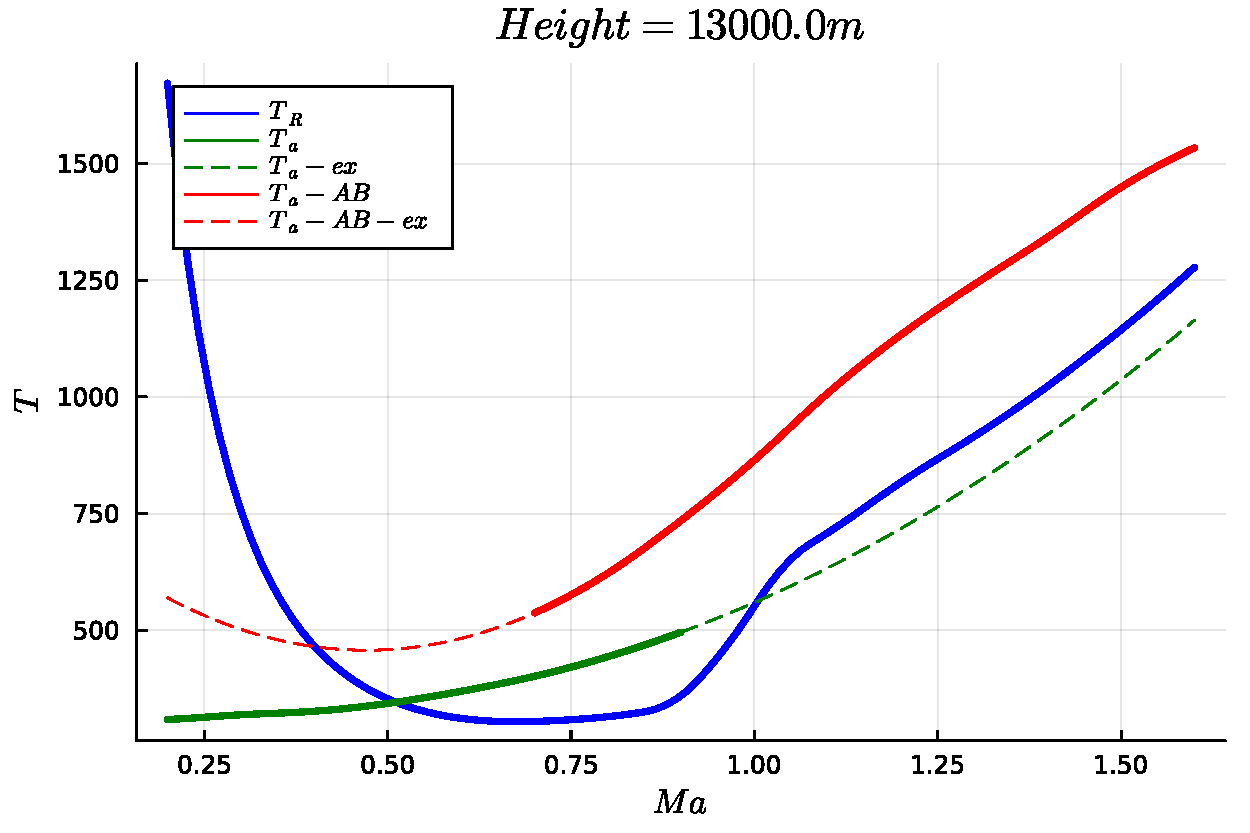
\includegraphics[width=0.25\textwidth]{image/ch4/h_TaTR_Ma14.pdf}
    }
    \subfloat[$h=14km$]{
        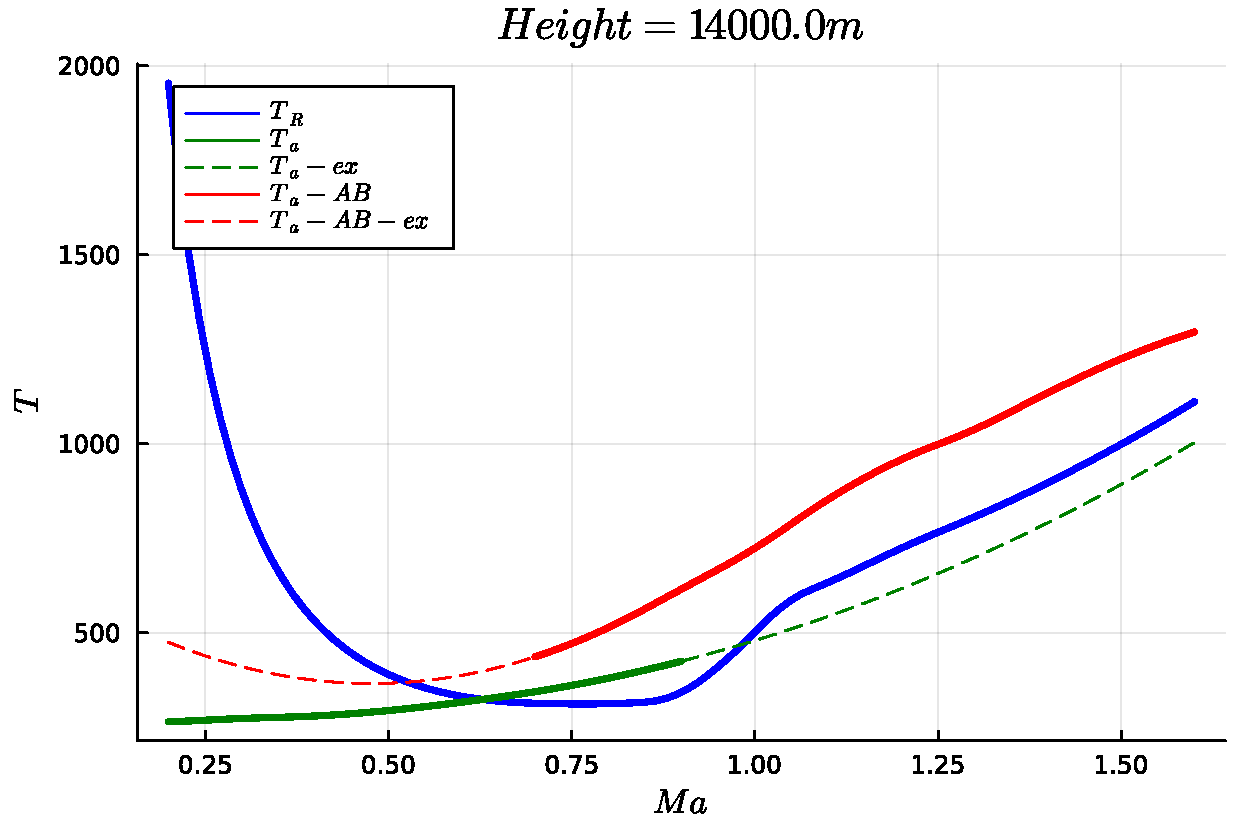
\includegraphics[width=0.25\textwidth]{image/ch4/h_TaTR_Ma15.pdf}
    }
    \subfloat[$h=15km$]{
        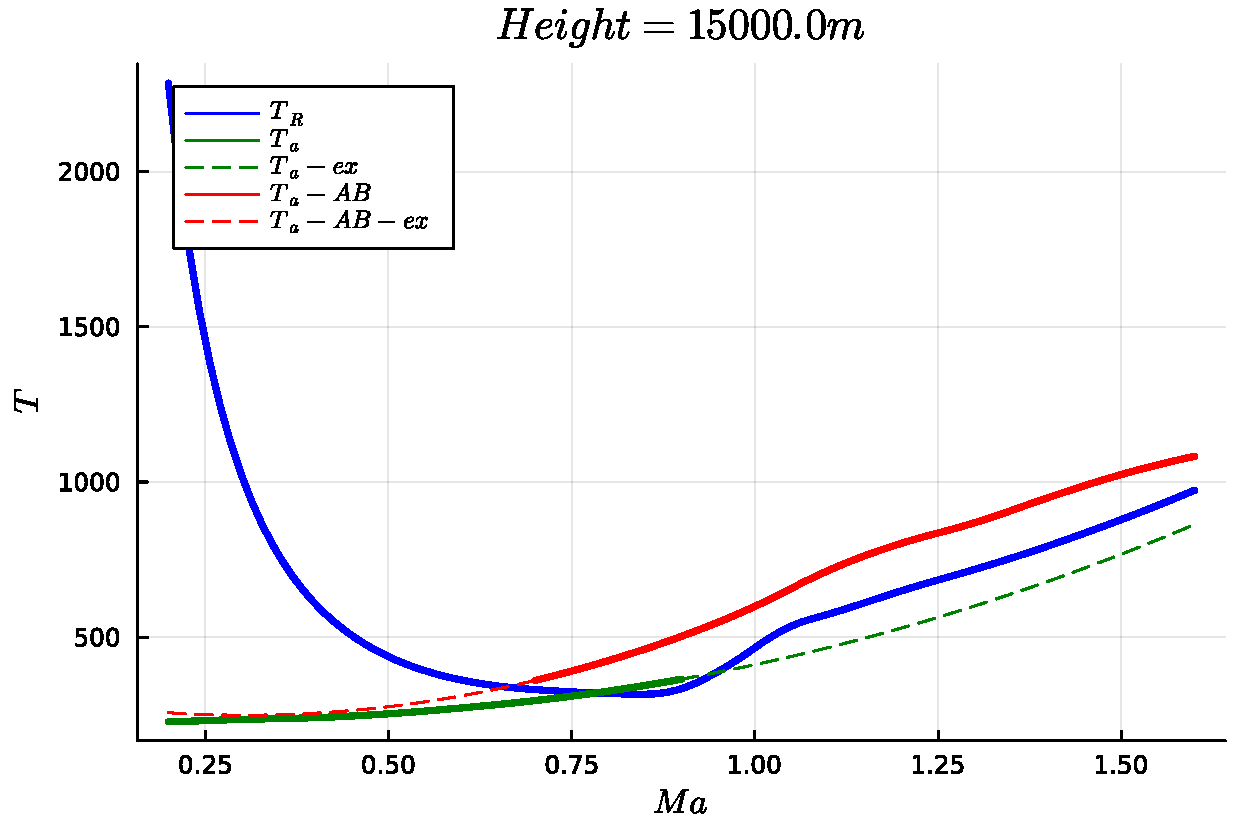
\includegraphics[width=0.25\textwidth]{image/ch4/h_TaTR_Ma16.pdf}
    }
    \caption{不同高度下可用推力$T_a$与需用推力$T_R$与飞行马赫数$Ma$的关系}
    \label{不同高度下可用推力与需用推力与飞行马赫数的关系}
\end{figure}


图\ref{不同高度下可用推力与需用推力与飞行马赫数的关系}中,
展示了在不同高度情况下,
可用推力$T_a$(加力与不加力),与需用推力$T_R$随着飞行马赫数$Ma$变化的关系。
其中蓝色实线表示需用推力$T_R$,
绿色实线表示不加力情况下的可用推力$T_a$,
绿色虚线表示不加力情况下的可用推力$T_a$外插;
红色实线表示加力情况下的可用推力$T_a$,
红色虚线表示加力情况下的可用推力$T_a$外插。

可以发现随着高度增加,
整体而言可用推力曲线随着高度增加不断在往蓝色的需用推力曲线逼近,
这也是该飞机(飞行器)逼近升限(即可用推力逐渐不足以满足需用推力)的趋势。